% last updated in April 2002 by Antje Endemann
% Based on CVPR 07 and LNCS, with modifications by DAF, AZ and elle, 2008 and AA, 2010, and CC, 2011; TT, 2014; AAS, 2016

\documentclass[runningheads]{llncs}
\usepackage{graphicx}
\usepackage{amsmath,amssymb} % define this before the line numbering.
\usepackage{ruler}
\usepackage{color}
\usepackage[width=122mm,left=12mm,paperwidth=146mm,height=193mm,top=12mm,paperheight=217mm]{geometry}

\newcommand{\commentJP}[1]{\textcolor{blue}{[JP: #1]}}
\newcommand{\KL}{\mathop{\textrm{KL}}}

\begin{document}
% \renewcommand\thelinenumber{\color[rgb]{0.2,0.5,0.8}\normalfont\sffamily\scriptsize\arabic{linenumber}\color[rgb]{0,0,0}}
% \renewcommand\makeLineNumber {\hss\thelinenumber\ \hspace{6mm} \rlap{\hskip\textwidth\ \hspace{6.5mm}\thelinenumber}}
% \linenumbers
\graphicspath{ {../images/} }
\pagestyle{headings}
\mainmatter
\def\ECCV16SubNumber{***}  % Insert your submission number here

\title{Hierarchical Object Representation based on a Sparse Autoencoder Network} % Replace with your title

\titlerunning{ECCV-16 submission ID \ECCV16SubNumber}

\authorrunning{ECCV-16 submission ID \ECCV16SubNumber}

\author{Anonymous ECCV submission}
\institute{Paper ID \ECCV16SubNumber}


\maketitle

\begin{abstract}

\dots
\keywords{Hierarchical Representation, Sparse Autoencoder Network, Depth Inference}
\end{abstract}


\section{Introduction}

Visual object recognition and categorization has many potential applications, enabling scene interpretation, semantic visual retrieval, and cognitive robotics. Furthermore, efficient object representations can be useful in a number of robotic application domains, such as object manipulation by a robotic arm, including tasks such as loading and unloading a dishwasher, grasping objects or opening a door. 

However, obtaining an efficient object representation is difficult due to high intra-class variation in shape, appearance and pose, but also due to illumination changes, occlusions or clutter. One approach useful for dealing with these limitations is to use a hierarchical object representation, which provides a compact representation on different levels of abstraction, provides object part shareability between different object categories and can cope with incompleteness produced by occlusions.

In recent years, many approaches have been proposed for object class detection using 2D features from a single view, such as the deformable part model \cite{Felzenswalb2010}, but also multi-view based methods which are useful at predicting not only the category but also the pose of an object in a scene \cite{Teney2014}. Furthermore, the availability of depth sensors such as Kinect had a great impact on the rapid development of algorithms for construction and acquisition of view-based 3D object models. Employing view-based 3D models for object recognition is useful, as they capture the intrinsic geometric structure of objects and provide a compact object representation \cite{Liebelt2010}. 

Provided that 2D and view-based 3D information are complementary, we aim to combine them in an efficient manner using a hierarchical representation, enabling improved recognition performance and inference of view-based 3D object parts given observed 2D parts. 

There are different fusion methods available, such as early-level fusion where different features are concatenated at an early stage, or decision-level fusion in which recognition is performed individually for each input channel and the final decision is taken by combining the independent results, using different criteria such as taking the maximum or using a weighted average \cite{Mahmoudi2013}.

These methods are insufficient for our goal, as we aim to take advantage of the correlations between 2D and view-based 3D information not only at the beginning or at the end of the recognition process, but to model them in a hierarchical manner, by considering relationships between parts in the 2D and view-based 3D hierarchies. Even though there are works which consider the relationships between 2D and 3D visual information, to the best of our knowledge, there is no other work which investigates this problem using a hierarchical modeling approach.

Therefore, in this work, we propose using both 2D and view-based 3D primitives, constructed using hierarchical representations, in which the effect of low-level visual features on higher-level entities is learned, leading to detection of object models in a scene and cross-hierarchy inference. 

The principles of hierarchy construction for both 2D and view-based 3D data are similar and are learned using sparse autoencoder networks. The relations between the two types of information are captured using an efficient probabilistic model. The model provides better inference, by reinforcing the evidence provided by one input channel with that from the other. Furthermore, it can be employed in the case of missing observations, inferring the most likely view-based 3D primitives from the observed 2D ones and vice-versa. 

In the following section we present a review of related work, while in Section~\ref{sec:learning} we introduce our hierarchical model for object representation using the two available data types, 2D intensity-based shape information and 3D view-based depth data. Next, in Section~\ref{sec:analysis} we present our method for capturing correspondences between 2D and view-based 3D primitives. The experimental results are introduced in Section~\ref{sec:results} and conclusions are formulated in Section~\ref{sec:conclusions}.

\section{Related Work}
\label{sec:related_work}  

One approach towards fusing 2D and 3D information consists of projecting a 3D shape into 2D and finding a set of meaningful multi-view 2D projections \cite{WangGWC0C13}, an option supported by Fleming and Singh \cite{Fleming2009} who argue that human perception of 3D shapes is based on 2D observations. The relation between 2D and 3D is exploited for 3D shape segmentation. First, the 2D projections of a 3D shape are labeled, then they are transferred to the 3D shape via back-projection, while finally the integration of multiple labels is done for obtaining a unified segmentation. Projection of 3D information into 2D as a means to recognize 3D objects and their pose is not new in computer vision and has been investigated also by Cyr and Kimia \cite{Cyr2001}. This approach is justified by the simplification of the problem, obtained by working in a low-dimensional space and by making use of the bigger volume of 2D image data available in the online environment. The disadvantages of this method reside in the complexity of the process, which requires manual labelling of parts, an assumption regarding the upright orientation of objects, as well as a slightly worse performance on articulated objects in comparison with rigid objects.

Another approach for capturing 2D to view-based 3D correlations is described by Cheng et al.~\cite{Cheng2010}. This work assumes that edge information in an image has a high probability of also being an edge in the depth map. Next, an image is divided into blocks and depth is assigned based on neighbourhood information and smoothed using bilateral filtering.

An adaptive fusion approach of 2D and 3D features is proposed by Arca et al.~\cite{Arca2007} with an application in face recognition. The integration of the two modalities is beneficial, as 2D features are more precise at capturing facial details, while 3D features are more robust under pose or lighting variations. The two types of features are fused at an early stage, while in the recognition process, only the most reliable features are used. Discarding of unreliable features is achieved using a matching criterion, which assigns weights based on a similarity measure. The same topic is investigated also by Soltana et al.~\cite{Soltana2010}, where the fusion strategy consists of an offline and an online weight learning process. In both cases the most relevant weights of all the scores for each sample in each modality is automatically selected.

3D object retrieval based on a 2D image represent another source of inspiration for linking 2D and 3D information. Eitz et al.~\cite{Eitz2012} propose using a sketch representation based on optimized Gabor filters, followed by a bag-of-words approach. The feature extraction technique can be further refined into a hierarchical representation using concepts proposed by Dai et al.~\cite{Dai2014}, which guide the learning of a dictionary of templates in an unsupervised manner. Each template is a composition of Gabor wavelets which are allowed to shift their location and orientation relative to each other. The invariance property is achieved using the active basis model \cite{Wu2010}.

The review of work dealing with 2D and view-based 3D information showed that fusing them is beneficial, while great care needs to be given to challenging issues such as conflicting data, outliers and noise, or data registration and correlation assessment. Without a proper pre-analysis of all these issues, the success rate of the fusion algorithm can be affected. 

In the next section, we introduce our proposed hierarchical object representation model.  

\section{Hierarchical Object Representation} 
\label{sec:learning}    

Our goal consists of matching 2D and view-based 3D parts in order to permit inference of 2D parts from observed view-based 3D parts and vice-versa and also to achieve better object recognition and/or object pose recognition accuracy.  

In order to obtain 2D and 3D-view based object parts at different levels of granularity, we propose using a hierarchical model which enables binding of parts at different levels. A hierarchical representation has advantages such as capturing exponential variability in a compact way and allowing fast inference.

The reason for building a new hierarchical model, instead of using existing models, is that we need a consistent method for forming parts for both modalities (2D intensity and 3D view-based), parts which need to share the same receptive field, otherwise correlations might only partially reflect the real relationships between the two information channels.

The principles for forming the hierarchical object representations are consistent for both 2D and 3D view-based data, where the size of the receptive field is gradually increased at each layer, up to the top layer which is sufficiently large to represent the whole object. Therefore, we will only describe the learning process for one type of data, namely 2D information. To obtain an object representation robust to illumination changes we use 2D shape information, obtained by applying an edge detection algorithm to the 2D intensity images.

The input used for learning the 2D hierarchical representation is a set $\mathcal{Z}$ of training edge images $Z^i \in \mathcal{Z}, i=1,\ldots,|\mathcal{Z}|$, represented\footnote{Here and in the following, superscripts always constitute upper indices; their use as powers will be indicated explicitly unless unambiguously clear from the context.} as a set of vectorized patches $Z_j$, i.e.,
$Z^i=\{Z_1,\ldots,Z_j,\ldots,Z_{|Z^i|}\}$\commentJP{Don't the $Z_j$ require an upper index $i$, i.e., $Z_j^i$?}, where each image patch
$Z_j=[z_{j1},\ldots,z_{jk},\ldots,z_{jn^2}]^T \in R^n$ is centered around an edge pixel $z_{jk}$. The size $n$ of an image patch is the size of the corresponding receptive field at the first layer, with $R_f^1=n^2$\commentJP{I corrected $n$ to $n^2$ in $Z_j$ above; please check. What is the subscript $f$? Just eliminate it everywhere.}, while the number of patches of each edge image $|Z^i|$ is given by the number of edges \commentJP{What exactly was $edgeNr$ intended to represent?} divided by the sampling rate \commentJP{what is the \emph{sampling rate}?}. The total number of patches used in the training phase is given by $|Z_*|=\sum_{i=1}^{|\mathcal{Z}|} |Z^i|$.

The first layer is learned using a sparse autoencoder algorithm, which is one approach to automatically learn features from unlabeled data and proved to be suitable not only for computer vision, but also for a range of problems including text, audio, etc. An autoencoder network is an unsupervised learning algorithm which applies backpropagation, setting the target values to be equal to the input values, as depicted in Figure \ref{fig:autoencoder} below. Therefore, one practical application is to use it for reconstruction. 

\begin{figure}
\begin{center}
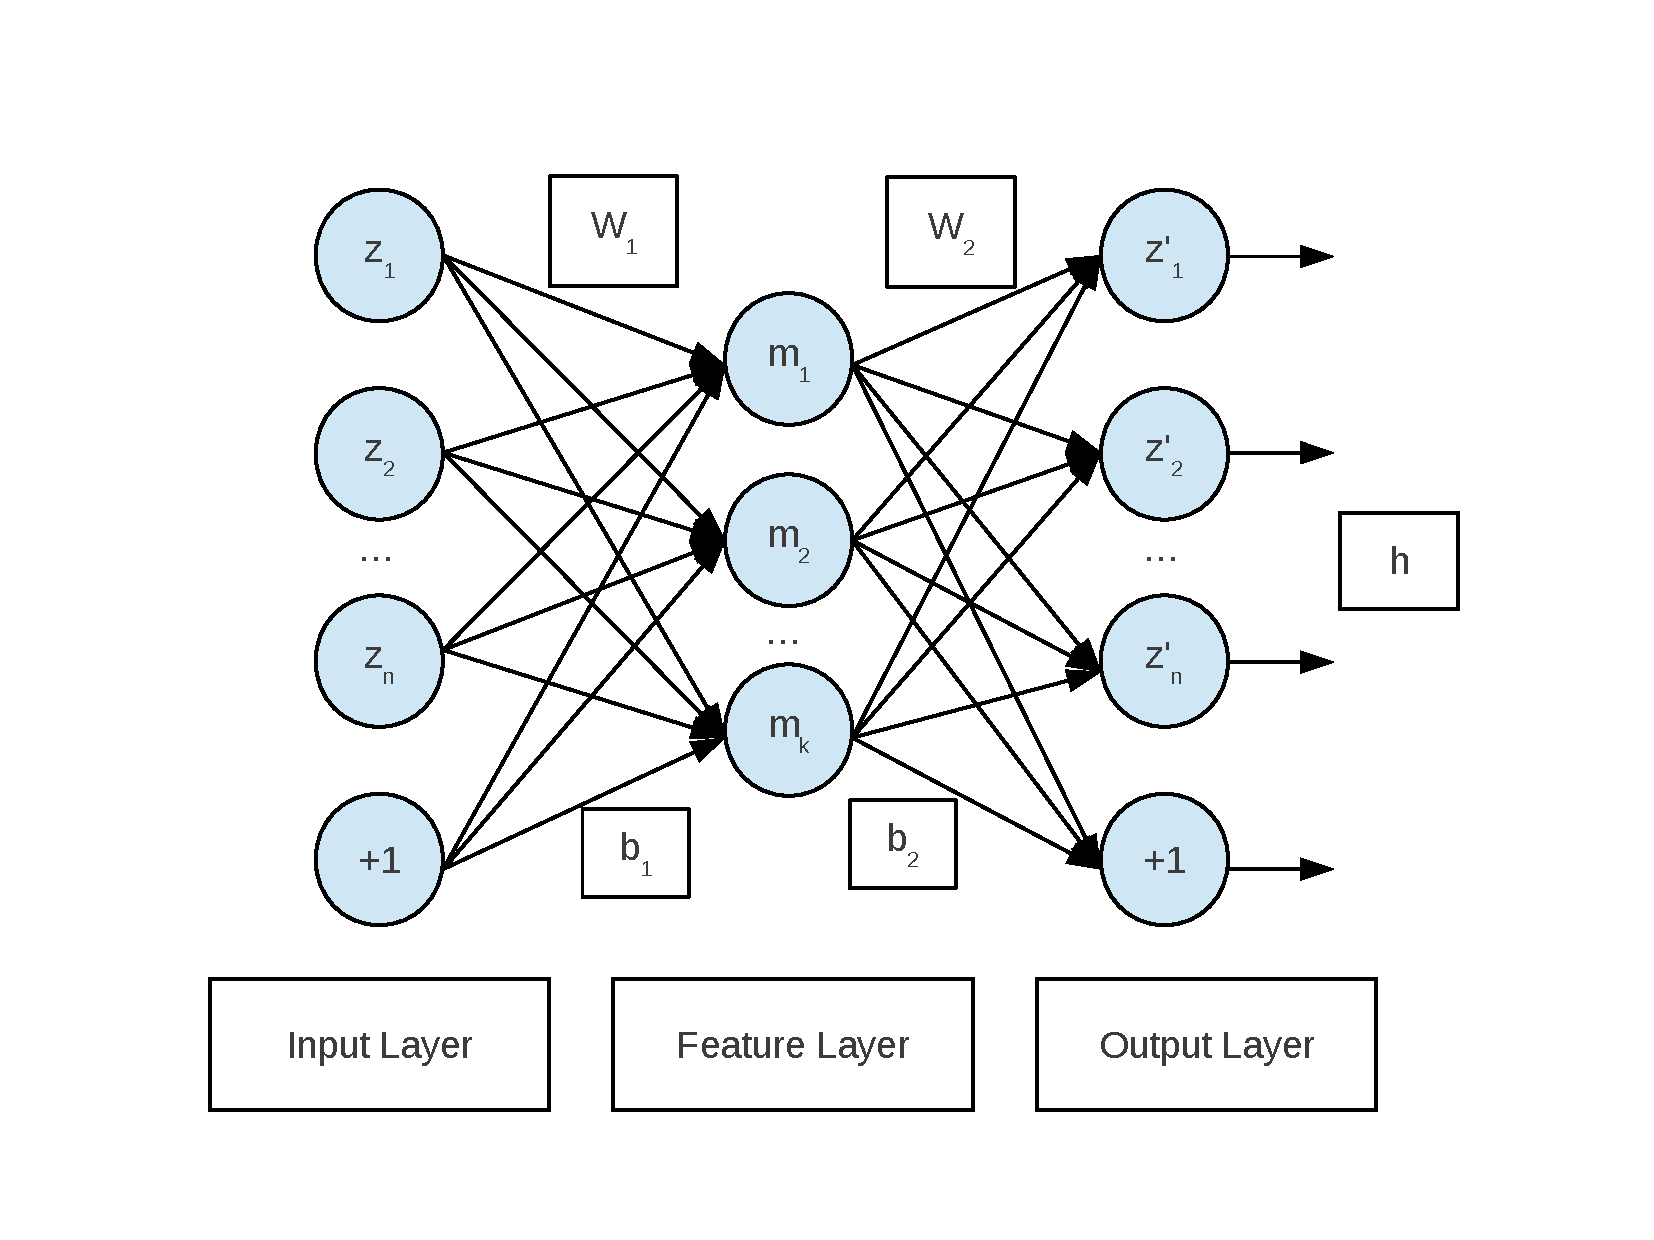
\includegraphics[width = 0.8\textwidth]{autoencoder}
\end{center}
\caption{Example of an autoencoder network, where the function $h$ learns an output $z'$ similar to the input $z$.}
\label{fig:autoencoder}
\end{figure}

The function used to map the input data $Z_j\in R^n$ is the function
\begin{equation}
 h(\theta,j)= g(W_2 g(W_1 Z_j+b_1)+b_2)
\end{equation}
which uses a set of linear combinations of the model parameters 
$\rho=(W_1,W_2,b_1,b_2)$ and a non-linear activation function $g$.

The sizes of the matrices $(W_1,W_2)$ and bias vectors $(b_1,b_2)$ are defined according to the vision task, which in our case is a reconstruction task. Therefore, given a desired number of features $k$ to be obtained, $W_1$ is of size $k\times n$, $W_2$ is of size $n\times k$, $b_1$ is of size $k$, and $b_2$ is of size $n$. The optimum number of features $k$ can be found experimentally, e.g.\ via cross-validation, to minimize the reconstruction error.

For the activation function $g$ there exist several options such as the sigmoid function
\begin{equation}
  g(z)=\frac{1}{1+\text{e}^{-z}}
\end{equation}
or the hyperbolic tangent
\begin{equation}
  g(z)=\tanh z=\frac{\text{e}^z-\text{e}^{-z}}{\text{e}^z+\text{e}^{-z}}.
\end{equation}
In the current implementation we chose to use the sigmoid function, as its range is $[0,1]$ which is suitable for image data, while the $\tanh$ function has a range of $[-1,1]$.

Learning the model parameters $\rho=(W_1,W_2,b_1,b_2)$ can be done using a batch gradient descent method, where the cost function $J$ can be defined to minimize the reconstruction error and will be trained on the data itself:
\begin{equation}
   J(\theta,j)=\left\|h(\theta,j)-Z_j\right\|_2^2 + \alpha W^2
\end{equation}
\commentJP{What is $W^2$?}
where the second term of the function is a regularization term that tends to decrease the magnitude of the weights---which helps to prevent overfitting---and the parameter $\alpha$ controls the relative importance of the two terms.
 
Furthermore, by placing different constraints on the cost function, such as limiting the number of hidden units, we can obtain a compressed representation of the input data. A sparsity constraint will force most of the hidden units to be inactive most of the time. By inactive, we mean the neuronal activation value is close to 0, while active means their value is close to 1. The new cost function is defined as
\begin{equation}
J_{\textrm{sparse}}(\theta)=J(\theta)+\beta \KL(\rho,\rho')
\end{equation}
where $\rho$ is the mean activation of the hidden units, and $\rho'$ is a sparsity parameter which is usually a small value close to zero. By minimizing the KL divergence, we thus force $\rho$ to be close to zero. In other words, we force most of the hidden units to be inactive.

After learning the model parameters, we want to obtain a discrete set of parts. This goal is achieved by clustering in the space of feature vectors formed of hidden unit activations. For each input patch $Z_j$, we obtain a feature vector
\begin{equation}
a_j=W_1Z_j+b_1, \;j=1,\ldots,|Z_*|.
\end{equation}
The output of the clustering method is a codebook
\begin{equation}
C^1=\{C_1,\ldots,C_i,\ldots,C_{M^1}\}
\end{equation}
which represents the set of parts at the first layer $\Gamma^{1}$. 

The number of clusters $M^l, l=1,\ldots,L_{2D}$ (where the number of layers for the 2D representation is $L_{2D}$) and the clustering method ($k$-means, agglomerative clustering, hierarchical clustering) represent two more design choices. These can be made based on experiments so as to find the optimum number of parts at each layer $l$. 

The input to the second layer is a set of patches $Z_j^2=\{a_1,\ldots,a_i,\ldots,a_{p^2}\}$, obtained by concatenating  $p^2$ overlapping feature vectors $a_i$ introduced in (6), extracted at different positions inside the specified receptive field at the second layer of twice the size, $R_f^2=2R_f^1$. The number $p^l$ of overlapping sub-parts considered at each layer represents another design decision.

We chose to optimize the parameter values based on minimizing the reconstruction error at each layer $l$. For this purpose, we considered the relative root mean square reconstruction error \cite{Chai2014}, which for one input image/feature patch $Z_j^l$ on layer $l$ is
\begin{equation}
 r_j^l = \frac{\left\|h^l(\theta,j)-Z_j^l\right\|_2}{\left\|Z_j^l\right\|_2},
\end{equation}
and the overall reconstruction error for a layer $l$ is
\begin{equation}
  r^l = \frac{1}{|Z_*^l|} \sum_{j=1}^{|Z_*^l|} r_j^l,
  \label{eq:r}
\end{equation}
where $|Z_*^l|$ is the number of patches on layer $l$.

The same learning method as described above is used to obtain the model parameters $\rho^2=(W_1^2,W_2^2,b_1^2,b_2^2)$ at the second layer, while the set of parts $\Gamma^{2}$ is obtained by clustering the feature vectors formed of activations at the second layer:
\begin{equation}
a_j^2=W_1^2Z_j^2+b_1^2, \;j=1,\ldots,|Z_*^2|
\end{equation}
where $|Z_*^2|$ is the number of extracted patches on the second layer.
\commentJP{You used $nr(\cdot)$ before, and here you used $N$.  Aren't they the same? Or is there a difference between the patch counts? Is my use of $|Z_*^{\cdot}|$ consistent?}

Next, all the other layers in our hierarchical representation, up to the top layer $L_{2D}$, are learned in an iterative manner as described above, where the input to each layer $l$ is given by the activations of the hidden units learned on patches from the previous layer $l-1$. This hierarchical approach is useful for capturing non-linear dependencies in the input data and models them iteratively, from low-level image patches up to the object level.

\commentJP{This section becomes very long, and the reader tends to lose track of where s/he is.  Consider dividing it into subsections with explicit titles.}

For optimizing the construction of the hierarchical representation, we decided to use supervised information on the last two layers. This design choice leads to the formation of category-specific parts \commentJP{which layers?}, view-specific parts at layer $L_{2D}-1$, and category-specific parts at the last layer. The learning process is the same as described above, with the only difference that image patches are selected only from images belonging to one object category, instead of coming from the entire database.    

Each layer will produce a set of weight vectors $W_1^l$ which compress the input information, while producing a useful representation. 

The set of model parameters at each layer $l$ is  given by
\begin{equation}
\theta^l = \{\rho^l,\Gamma^l,R_f^l\},
\rho^l=(W_1^l,W_2^l,b_1^l,b_2^l).
\end{equation}
\commentJP{Is there a reason why you mix set and tuple notation?}

The set of parts obtained at each layer $l\in\{1,\ldots,n_{2D}\}$ for the 2D $\{\Gamma^l\}$ and view-based 3D $\{\Omega^l\}$ hierarchical representations are depicted in Section~\ref{sec:results}.

An approach similar to that described above was proposed by Masci et al.~\cite{Masci2011}, where stacked autoencoders are trained in a similar fashion, one layer at a time, and each layer receives as input the latent representation of the layer below. The main difference from that work, addressed in our approach, is the cross-hierarchy prediction power which is achieved by discretizing the responses of each layer into a set of parts, using clustering techniques. This step enables efficient inference of parts from one hierarchy, given observed parts in the other hierarchy. In the next section we present our model for binding the two hierarchical representations for 2D and view-based 3D data.
 
\section{Establishing correspondences between 2D and 3D view-based hierarchical representations}
\label{sec:analysis}

We build the 2D and the view-based 3D hierarchical representations on similar learning principles and their parts encode on each layer the same spatial locality $R_{f(2D)}^l=R_{f(3D)}^l$, while the difference consists in the different type of information they encode, edges and depth.
	
Furthermore, the two hierarchies are trained on the same object models, consisting of both 2D edge images and the corresponding depth images or point clouds.  

The hierarchical compositional 2D model is formed of $n_{2D}$ layers, each layer being composed of a number of 2D parts. 
As our main goal was to be able to do efficient inference across the two representations, we chose to use the same number of layers in both hierarchies, such as $n_{2D}=n_{3D}=n_h$.

We denote the $i^{th}$ part constructed at the $l^{th}$ layer of a  hierarchical vocabulary of 2D shapes as $\Gamma_{i}^{l}$, where $i \in \{1,\ldots,n_{l}\}, l \in \{1,\ldots,n_h\}$. The $j^{th}$ part constructed at the $l^{th}$ layer of the  hierarchical vocabulary of view-based 3D shapes as $\Omega_{j}^{l}$, where $j \in \{1,\ldots,n_{l}^{'}\}, {l} \in \{1,\ldots,n_h\}$. As the number of parts at a layer $l$ in each hierarchy can be different, we use the notation $n_l$ for the 2D case and $n_l^{'}$ for the view-based 3D parts. 

For establishing correspondences between the parts in the two hierarchies, we build a \emph{correspondence table} with row indices $(1,\dots,N)$, (where $N=\sum_{l=1}^{n_h} {n_l}$) corresponding to the 2D parts and columns indices $(1,\dots,M)$, where $M=\sum_{l=1}^{n_h} {n_{l}^ {'}}$) corresponding to the view-based 3D parts, as depicted in Figure~\ref{fig:fused-models} below. 

We will establish level-by-level correspondences between 2D and view-based 3D  parts (($\Gamma_{i}^l,\Omega_{j}^l$), $i \in (1,\ldots,n_l), j \in (1,\ldots,n_{l}^{'})$).

The correspondences between the two types of parts are build using an observation function $c^l$, which quantizes the co-occurrences of one 2D and a view-based 3D part and vice-versa at each layer. 

Next, we illustrate the parts binding mechanism in Figure \ref{fig:fused-models}.

\begin{figure}
\begin{center}
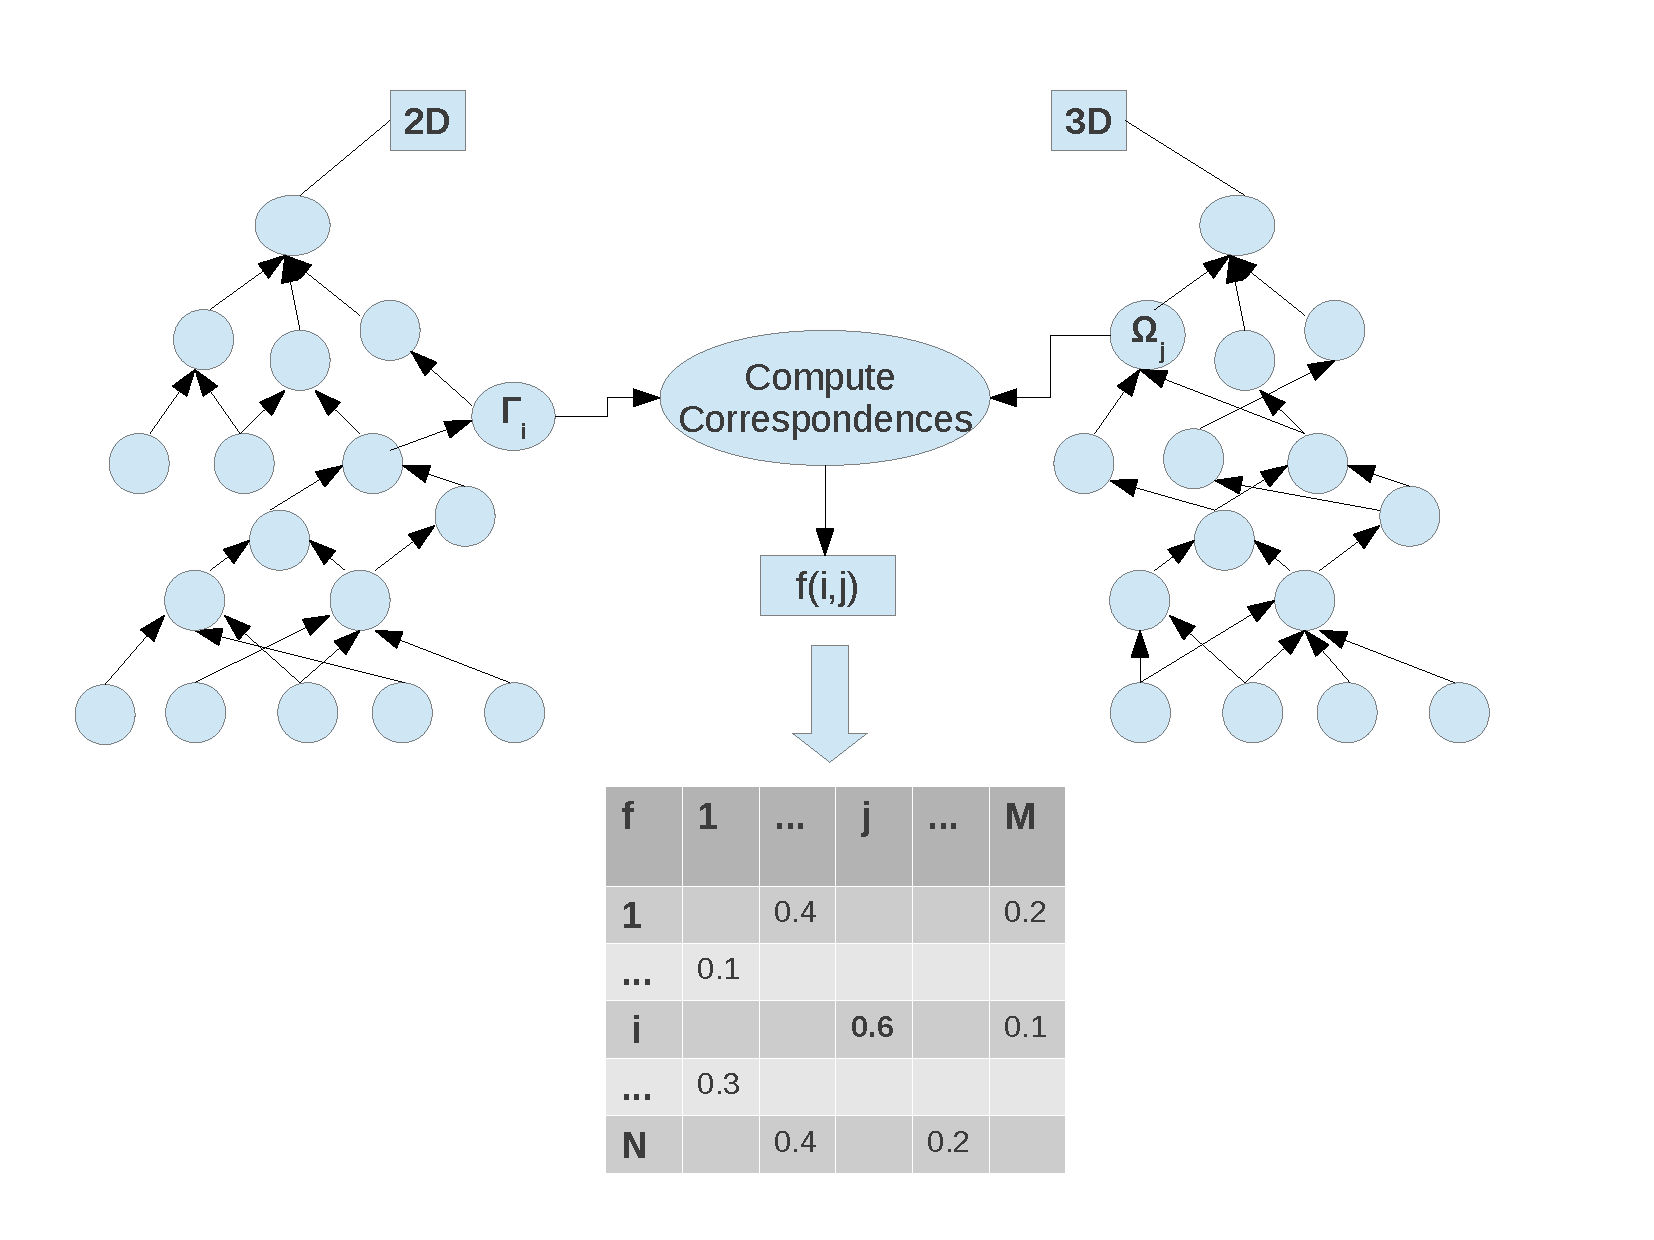
\includegraphics[width=0.9\textwidth]{Fused_representation}
\end{center}
\caption{Correspondences between the 2D and view-based 3D hierarchies.}
\label{fig:fused-models}
\end{figure}

To every correspondence $c^l(i,j)$, where $i$ is the index of the 2D part $\Gamma_i^l$ and $j$ the index of the view-based 3D part $\Omega_j^l$ on layer $l$, we assign a real value. As for each 3D/2D part there might be several 2D/3D parts corresponding to it, all associated correspondences will be activated. Therefore, the value $c^l(i,j)$ is computed as the joint probability of observing parts $\Gamma_i^l$ and $\Omega_j^l$ at the same spatial location:

\begin{equation}
  c^l(i,j) = P(\Gamma_i^l,\Omega_j^l). 
 \end{equation} 

In general, there will not be a one-to-one relation between 2D and view-based 3D parts, as the 2D parts are represented using edges and they can be correlated with depth parts which encode depth disparities on one side or the other one of the edge part and also can be correlated with internal depth edges. Still, the number of correlations will decrease for higher level parts, as more complex edge structures such as L, Y or T junctions are better at predicting the possible associated depth structures.

The correspondence table represents the set of possible correspondences over all sets of 2D and view-based 3D parts.  

Moreover, the joint probability table of 2D and view-based 3D parts can be used for performing inference of view-based 3D parts/2D parts coherently and transparently across the 2D and view-based 3D hierarchies.

Still, the inference process can be regraded from two perspectives, given the type of parts we want to predict, either 2D or 3D. 

Therefore, for he task of inferring a 2D part $\Gamma_i^l$ from an observed view-based 3D part $\Omega_j^l$ at layer $l$, we employ the conditional probability:

\begin{equation}
P(\Gamma_i^l \vert \Omega_j^l), i \in \{1,\dots,n_l\},
\end{equation}

operation, which will retrieve all 2D parts $\Gamma_i^l$ which are probable to be observed with the view-based 3D part $\Omega_j^l$. 

The relation to equation (12) is build using the Bayes rule such as:
\begin{equation}
P(\Gamma_i^l \vert \Omega_j^l)= \frac{P(\Gamma_i^l,\Omega_j^l)}{P(\Omega_j^l)}.
\end{equation}

Respectively, inference of a view-based 3D part $\Omega_j^l$ can be performed using the conditional probability:
\begin{equation}
 P(\Omega_j^l \vert \Gamma_i^l), j \in \{1,\dots,n_{l}^{'}\},
\end{equation} 
which permits retrieving all view-based 3D parts $\Omega_j^l$ which could be observed with the 2D part $\Gamma_i^l$. 

Furthermore, the relation to equation (12) is given by:

\begin{equation}
 P(\Omega_j^l \vert \Gamma_i^l)=\frac{P(\Omega_j^l,\Gamma_i^l)}{P(\Gamma_i^l)}.
\end{equation} 
 
The correspondence table introduced above can be considered as a starting point for different tasks, such as inferring view-based 3D parts from observed 2D parts, and respectively inferring 2D parts from observed view-based 3D parts, object recognition, object reconstruction, or pose estimation. 

Furthermore, the correspondence table can be used as a starting point for building better prediction models, such as training a classifier for predicting 3D view-based parts, given an observed 2D part, which takes into account not only the conditional probabilities across hierarchies, but also their associated feature vectors.

\subsection{Inference of View-based 3D Parts using 2D and 3D Hierarchical Compositional Models}
\label{sec:inference}

We propose a probabilistic model for performing inference in the view-based 3D hierarchy, by reusing the inference mechanism existing in the 2D hierarchy in combination with the joint probability table introduced above.

We use the assumption that parts in the view-based 3D hierarchy are formed by propagating evidence from lower levels to higher ones in a probabilistic manner. 

Next, we condition the probability of a view-based 3D part $\Omega_j^{l}$ at layer $l$ not only on the the sub-parts on the previous layer $l-1$, but also on the 2D parts that are probable to co-occur with it. We will replace the conditional probability:

\begin{equation}
 P(\Omega_j^{l} \vert \Omega_i^{l-1}), i \in \{1,\dots,n_{l-1}^{'}\},
\end{equation}
with:
\begin{equation}
 P(\Omega_j^{l} \vert \Omega_i^{l-1},\Gamma_k^l), i \in \{1,\dots,n_{l-1}^{'}\}.
\end{equation}

2D parts $\Gamma_k^l$ are retrieved using the joint probability table introduced in Section \ref{sec:analysis} and consist of the set of 2D parts which maximize the $P(\Gamma_k^l,\Omega_j^l)$. The threshold for part selection $\tau$, where $P(\Gamma_k^l,\Omega_j^l)>\tau$ is learned according to the purpose of the inference process.

Furthermore, according to Bayes rule we can estimate the conditional probability introduced in (18) as follows:

\begin{equation}
 P(\Omega_j^{l} \vert \Omega_i^{l-1},\Gamma_k^l) = \frac{P(\Omega_i^{l-1},\Gamma_k^l \vert \Omega_j^{l})P(\Omega_j^{l})}{P(\Omega_i^{l-1},\Gamma_k^l)}.
\end{equation}

For estimating the following conditional probability:

\begin{equation}
 P(\Omega_i^{l-1},\Gamma_k^l \vert \Omega_j^{l}) =  P(\Gamma_k^l \vert \Omega_j^{l},\Omega_i^{l-1}) P(\Omega_i^{l-1} \vert \Omega_j^{l}),
\end{equation}

we take into account the introduced definition of neighbourhood, which suggests that if the pairs of parts $(\Gamma_k^l,\Omega_j^{l})$ and $(\Omega_j^{l},\Omega_i^{l-1})$ are in the same neighbourhood and can be correlated, then the parts $(\Gamma_k^l,\Omega_i^{l-1})$ are conditionally independent, given part $\Omega_j^{l}$, as the correspondences between parts are established at the highest possible layers in the two hierarchies and therefore: 

\begin{equation}
 P(\Omega_i^{l-1},\Gamma_k^l \vert \Omega_j^{l}) =  P(\Gamma_k^l \vert \Omega_j^{l}) P(\Omega_i^{l-1} \vert \Omega_j^{l}).
\end{equation}

By introducing equation (21) into (19) we obtain:

\begin{equation}
 P(\Omega_j^{l} \vert \Omega_i^{l-1},\Gamma_k^l) = \frac{P(\Gamma_k^l \vert \Omega_j^{l})P(\Omega_i^{l-1} \vert \Omega_j^{l})P(\Omega_j^{l})}{P(\Omega_i^{l-1},\Gamma_k^l)},
\end{equation}

where the conditional probability $P(\Gamma_k^l \vert \Omega_j^l)$ can be obtained from equation (14) and $P(\Omega_i^{l-1} \vert \Omega_j^{l})$ can be computed using the initial conditional probability introduced in (17) as follows:

\begin{equation}
 P(\Omega_i^{l-1} \vert \Omega_j^{l}) = \frac{P(\Omega_j^{l}\vert \Omega_i^{l-1})P(\Omega_i^{l-1})}{P(\Omega_j^{l})}.
 \end{equation}

Finally, by introducing equation (23) into (22) we obtain:

\begin{equation}
 P(\Omega_j^{l} \vert \Omega_i^{l-1},\Gamma_k^l) = \frac{P(\Gamma_k^l \vert \Omega_j^{l})P(\Omega_j^{l} \vert \Omega_i^{l-1})P(\Omega_i^{l-1})}{P(\Omega_i^{l-1},\Gamma_k^l)}.
\end{equation}
  
The view-based 3D part prior $P(\Omega_i^{l-1})$ can be considered uniform or computed using the inverse frequency operator on an input database, which takes into account the part frequency across the database, while the joint probability $P(\Omega_i^{l-1},\Gamma_k^l)$ can be obtained from equation (16) presented in Section \ref{sec:analysis}.

The proposed model will be initialized with probabilities of 2D parts on the first layer of the 2D hierarchy. Next, the observations in the 2D hierarchy will be used to propagate information in the view-based 3D hierarchy and finally to obtain hypotheses about view-based 3D parts. 

Next, we analyze a set of statistical properties of the correspondences between parts in the 2D and view-based 3D hierarchies. This analysis will be used to obtain a better understanding of the benefits achieved by fusing them.

\subsection{Statistical Evaluation}
\label{sec:statistical}

The purpose of the statistical evaluation of the correspondences between the two information channels 2D and view-based 3D is to assess the relations which can be formed between them and furthermore, to draw conclusion regarding the efficiency of the inference process. 

For quantizing correspondences between parts in the 2D and view-based 3D hierarchies, we use several statistical measures.

First, we analyze on each layer $l$ the correspondences of each 2D/3D part, given the set of 3D/2D parts on that layer, by constructing a pdf over all computed conditional probabilities of that part. A peaked pdf suggests that the considered 2D/3D part can be matched successfully to a part or to a limited set of 3D/2D parts, while a multi-peak distribution indicates that more information is needed in order to predict a good matching. The pairs of parts which can be matched with a lower uncertainty between the two hierarchies, should be given a higher weight in the inference process, as they are better at predicting the unknown part in the other hierarchy.

Next, we compute the conditional entropy of 2D parts given 3D parts on layer $l$ and vice-versa, using the conditional probabilities introduced in equations (14) and (16). This measure computes the amount of uncertainty remaining in predicting 2D parts given 3D parts and vice-versa, thus helping us to determine which information, either 2D or 3D, is better at predicting the other type of information in the inference process. The analysis is performed for each layer in the 2D and view-based 3D hierarchical representations.

\begin{equation}
 H^l(\Delta^l|\Theta^l) = -\sum\limits_{j=1}^{n_l^{'}}P({\Omega_j^l})\sum\limits_{i=1}^{n_l}P(\Gamma_i^l|\Omega_j^l)\log P(\Gamma_i^l|\Omega_j^l), 
\end{equation}

\begin{equation}
 H^l(\Theta^l|\Delta^l) = -\sum\limits_{i=1}^{n_l}P({\Gamma_i^l})\sum\limits_{j=1}^{n_l^{'}}P(\Omega_j^l|\Gamma_i^l)\log P(\Omega_j^l|\Gamma_i^l),
\end{equation}
where $\Delta^l$ consists of all 2D parts $\{\Gamma_i^l, i \in (1,\ldots,n_l)\}$ and $\Theta^l$ consists of all the view-based 3D parts $\{\Omega_j^l, j \in (1,\ldots,n_l^{'})\}$ on layer $l$.

Moreover, we also analyze the mutual information of the parts in the 2D and 3D compositional representations on layer $l$, as a measure of the parts mutual dependence, by employing the joint probabilities introduced in equation (12).

\begin{equation}
 I^l(\Delta^l;\Theta^l) = \sum\limits_{j=1}^{n_l^{'}}\sum\limits_{i=1}^{n_l}P({\Gamma_i^l},\Omega_j^l)\log \frac{P({\Gamma_i^l},\Omega_j^l)}{P({\Gamma_i^l})P(\Omega_j^l)}.
\end{equation}

In the following section we provide the results of the performed statistical evaluation.

\section{Experimental Results}
\label{sec:results}

We learned and tested the proposed hierarchical representations for 2D and view-based 3D data on a set of object categories from the PaCMan dataset which is publicly available\footnote{\url{http://www.pacman-project.eu/datasets/}}. We depict in Figure \ref{database} a set of example images (edge and depth) used in the training phase. The dataset contains gray-scale and depth images generated from 3D models of 20 categories of various kitchen objects, each category containing on average 20 instances. Each object is captured at dense, regular viewpoint intervals, and we use all the 48 different viewpoints of an object instance, both in the training and testing phase.

\begin{figure}
\begin{center}
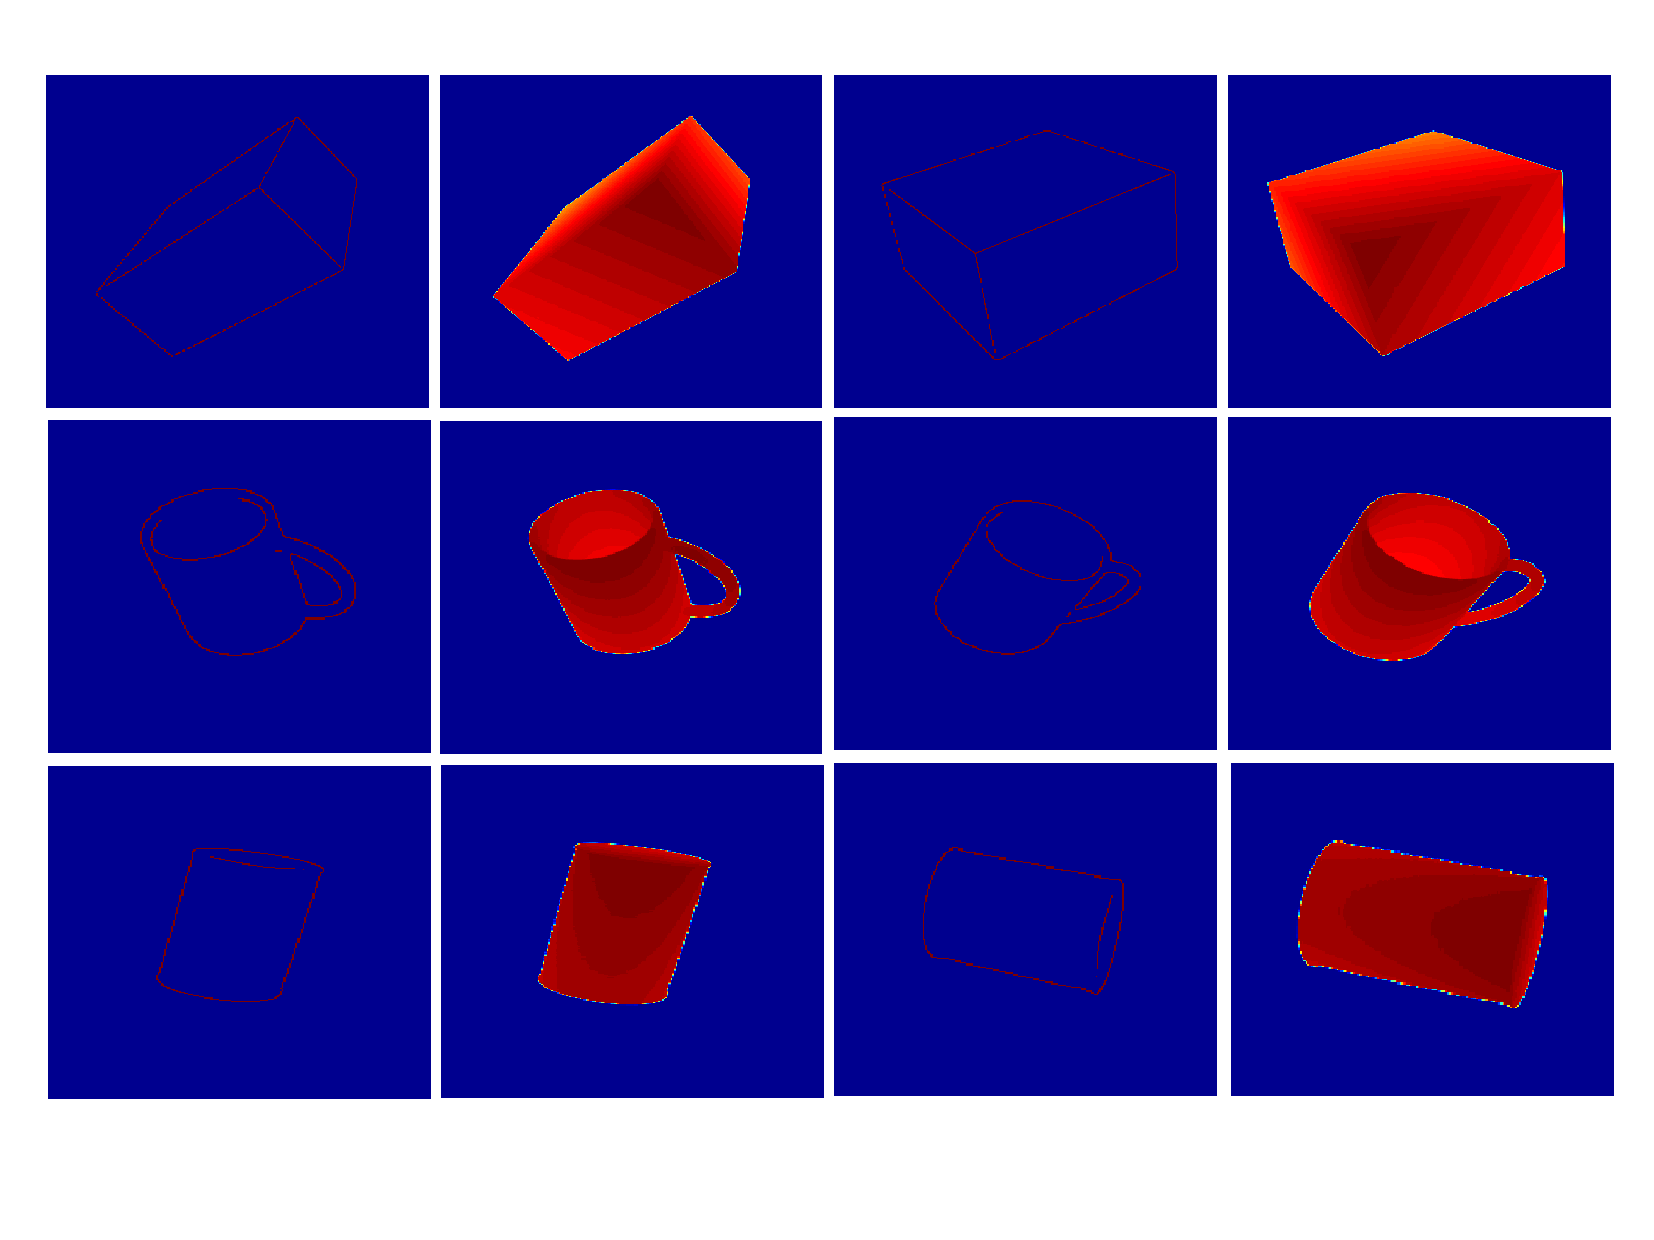
\includegraphics[width=0.6\textwidth]{database}
\end{center}
\caption{Examples of objects instances (box, mug, can) from the PaCMan database.}
\label{database}
\end{figure}

The number of constructed layers in a hierarchy depends on the size of the training objects and for the PaCMan dataset, the hierarchical representations are formed of five layers. 

One important issue consisted of finding the optimum number of parts on each layer for each representation, and apart from minimizing the reconstruction error introduced in (8), we also used the Davies-Bouldin (DB) index \cite{Bouldin97} as a method to assess the quality of the clustering process. The optimum number of parts $k$ on a layer $l$ is selected according to the minimum DB index. As the dimensionality of the feature vectors used in the clustering process is increasing on each layer, we applied a dimensionality reduction method such as PCA for obtaining a faster and more efficient selection of the optimum number of clusters.

Examples of learned parts on each layer of the two hierarchical representations and correspondences between them are depicted in Figure \ref{hierarchy}.

\begin{figure}
\begin{center}
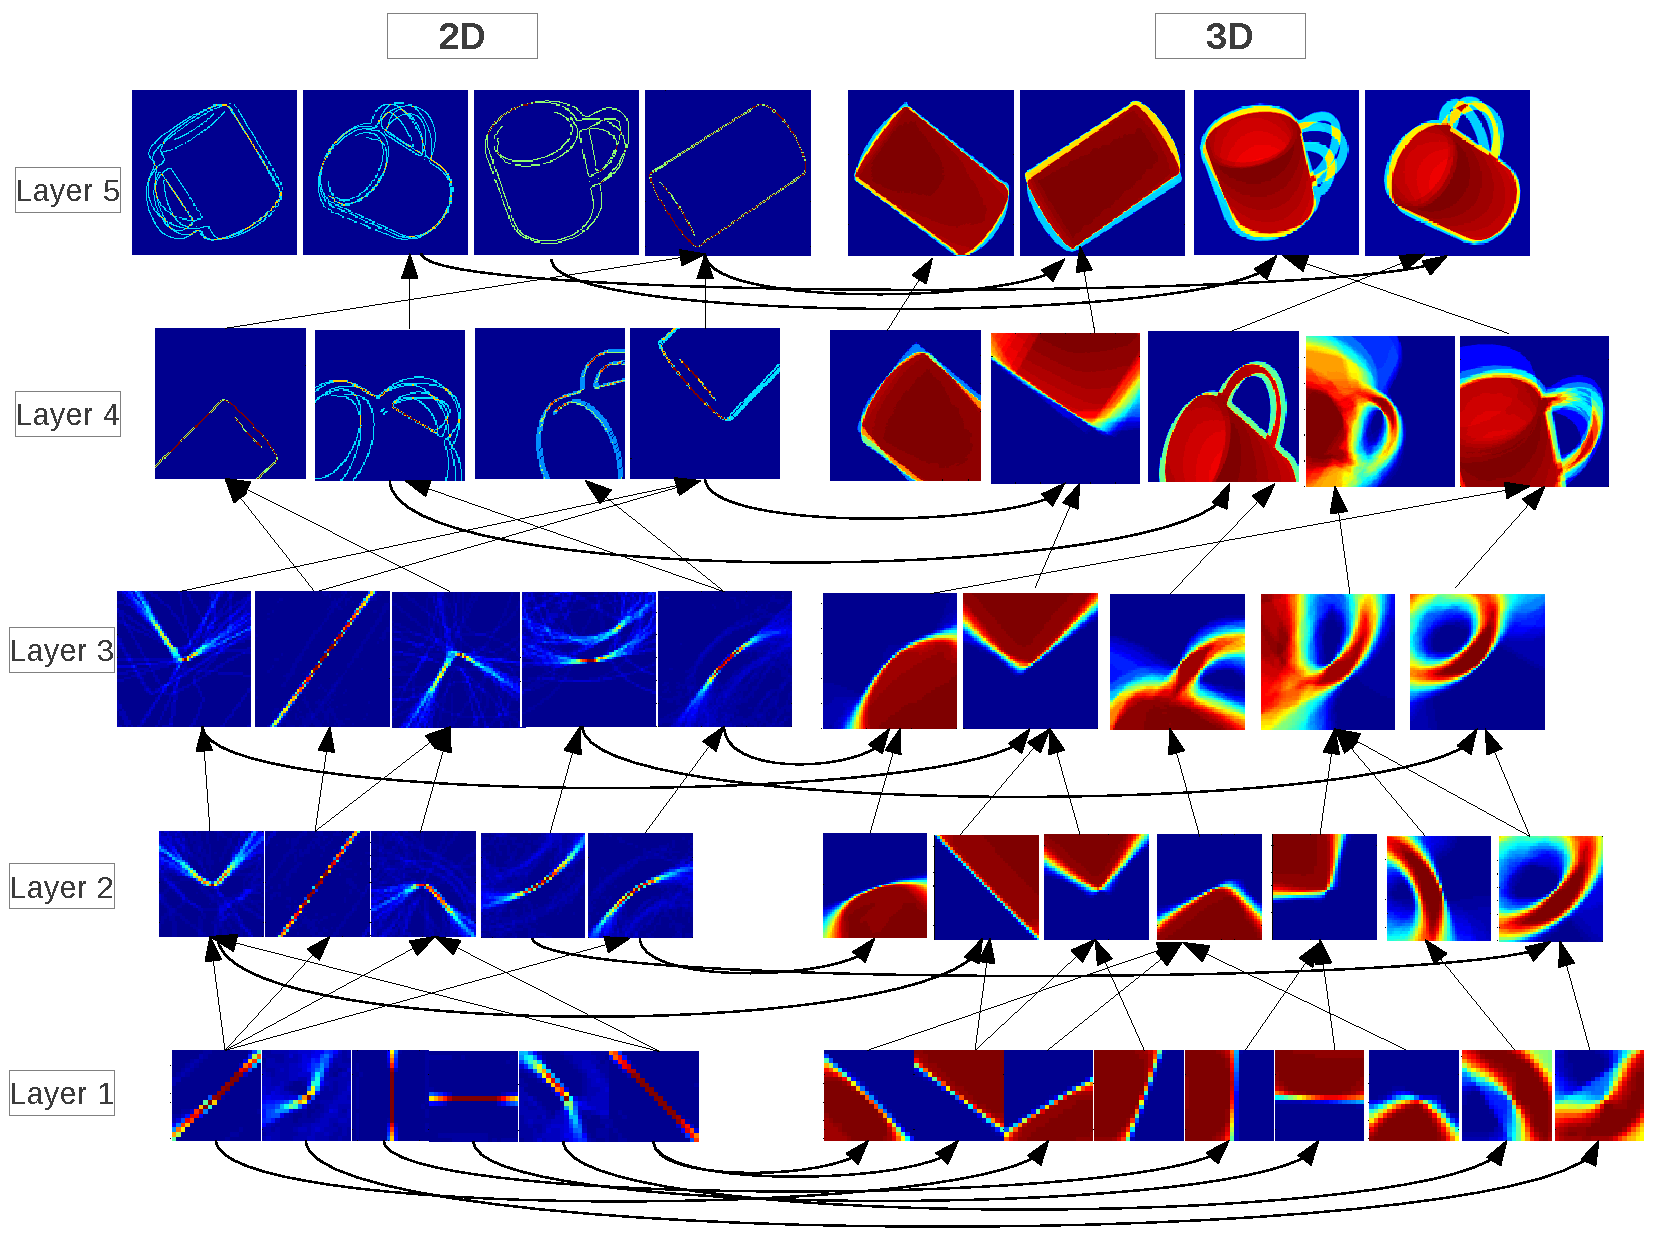
\includegraphics[width=0.8\textwidth]{hierarchy}
\end{center}
\caption{Examples of parts at each layer in the 2D and view-based 3D hierarchies and correspondences between them.}
\label{hierarchy}
\end{figure}

We present in Table 1 for each layer in the 2D and view-based 3D hierarchies, the optimum number of parts, the reconstruction error for each hierarchy and the part entropies introduced in section \ref{sec:statistical}. The reconstruction error is computed using an adaptation of the formula introduced in (8):

\begin{equation}
 r_j^l = \frac{\left\|\Gamma_m^l-Z_j^l\right\|_2}{\left\|Z_j^l\right\|_2}, \end{equation}
 
 where m is the index of best fitting part for the patch $Z_j^l$ at the layer $l$ which indicates the size of the receptive field $R_f^l$:
 
\begin{equation}
 m=min_{i=1}^{n_l}(\left\|\Gamma_i^l-Z_j^l\right\|_2).
\end{equation}

 \begin{table}
 \begin{center}
  \begin{tabular}{ | c | c | c | c | c | c | c |r |}
      \hline
      $Layers$  & $Size(\Delta^l)$ & $Err_{2D}$ & $H(\Delta^l)$ &  $Size(\Theta^l)$ & $Err_{3D}$ & $H(\Theta^l)$  \\ \hline
    $l_1$ &  130  & 0.32 & 4.78 & 100 & 0.53 & 4.2 \\ \hline
    $l_2$ &  400 & 0.49 & 5.74 & 400 & 0.42 & 5.64 \\ \hline
    $l_3$ &  400 & 0.63 & 5.68 & 500 & 0.37 & 5.97 \\ \hline 
    $l_4$ &  550 & 0.71 & 5.95 & 600 & 0.31 & 6.14 \\ \hline
    $l_5$ &   &  &  &  &  &  \\ 
    \hline
  \end{tabular}
\end{center}
\caption{Statistics of parts at Layers 1-5 in the 2D and view-based 3D hierarchies.}
\end{table}

Analysis of the results presented in Table 1, highlights two phenomena, the reconstruction error in the 2D case is increasing, while in the 3D case is decreasing from bottom layers to top ones. As the error is computed per pixel in a patch, a slight translation of an edge part will increase the error, while in the depth case, higher level structures are better at describing the data and therefore the error is decreasing. Regarding the part entropies at each layer, we notice a slight increase, which is caused by the increasing of the number of parts from bottom-up, having a direct impact on the part uncertainties when sampled from the underlying part probability distributions on that layer.

\begin{figure}
\begin{center}
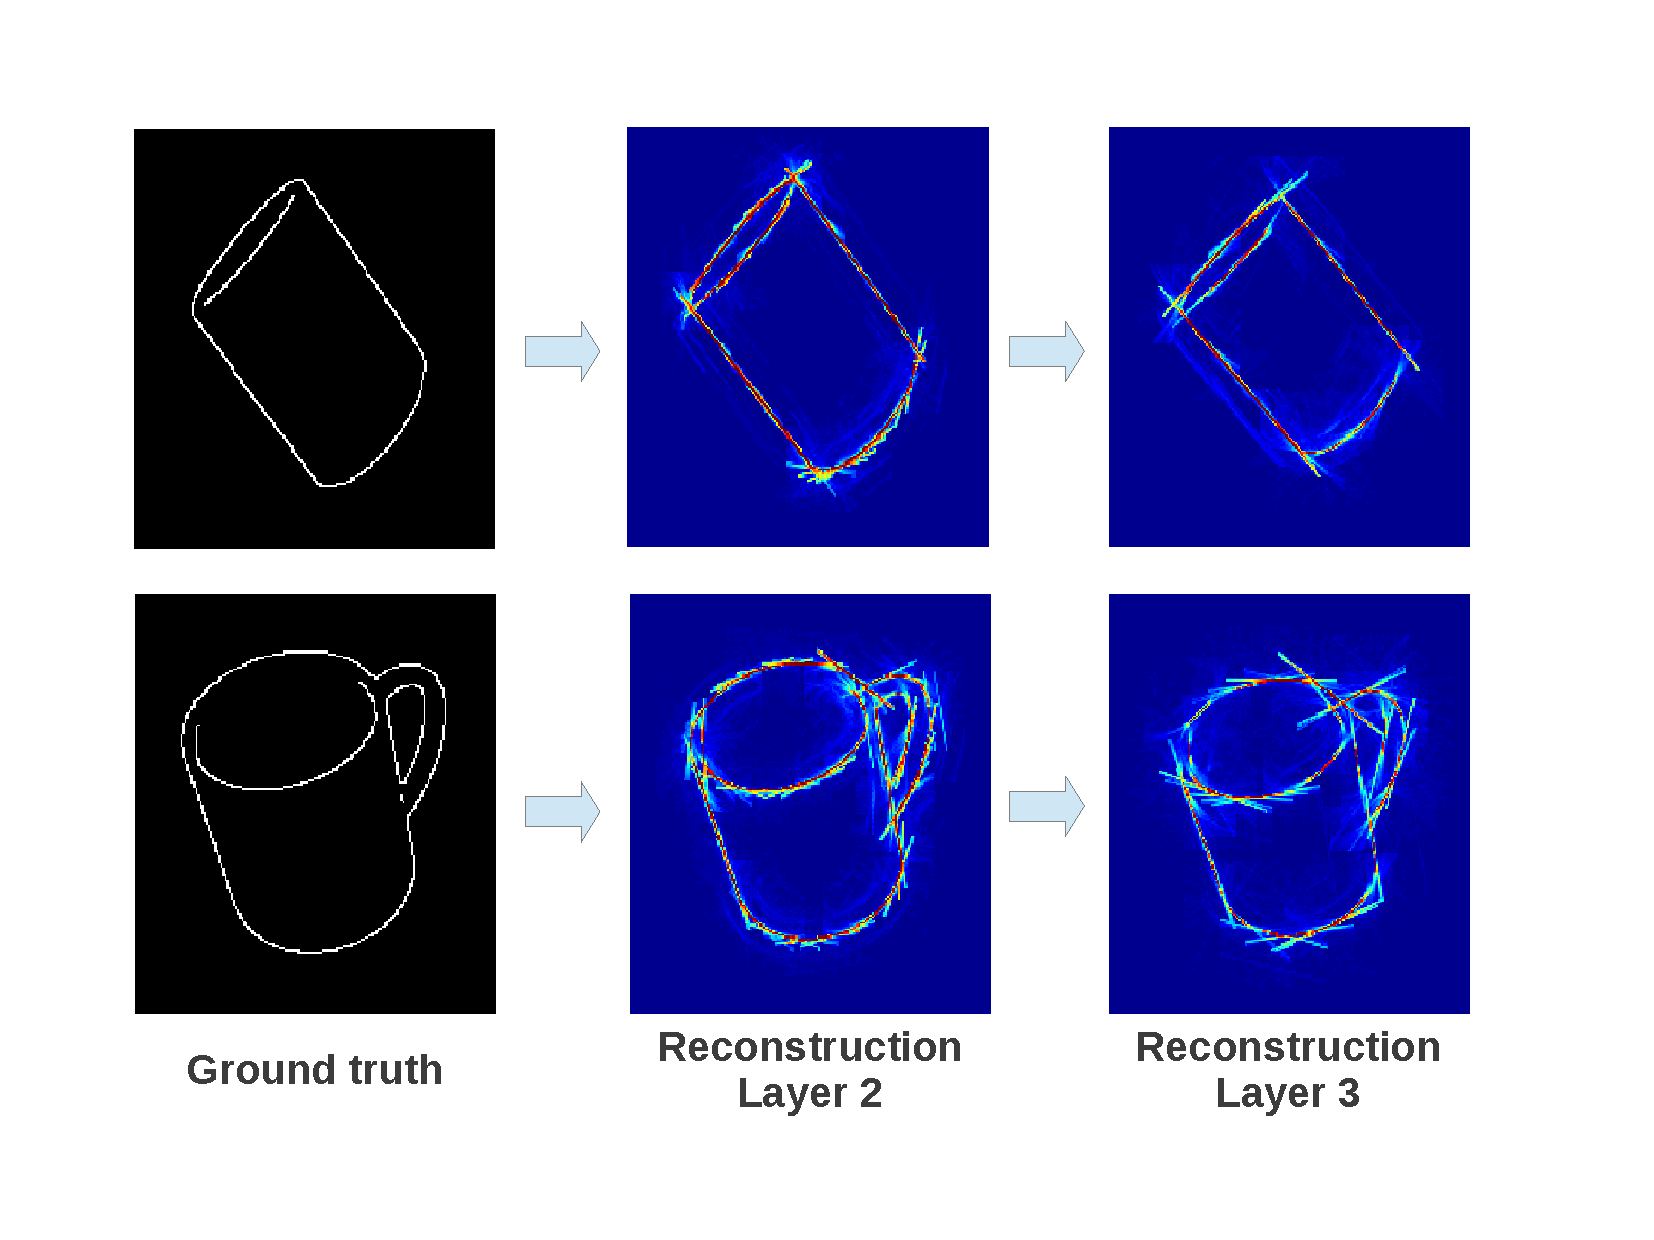
\includegraphics[width=0.7\textwidth]{reconstruction_edge}
\end{center}
\caption{2D reconstruction examples of a mug instance from different viewpoints at Layer 2-3.}
\label{reconstructionEdge}
\end{figure}

We present in Figures \ref{reconstructionEdge} and \ref{reconstructionDepth} several examples of reconstruction for both hierarchical representations at different layers. 

\begin{figure}
\begin{center}
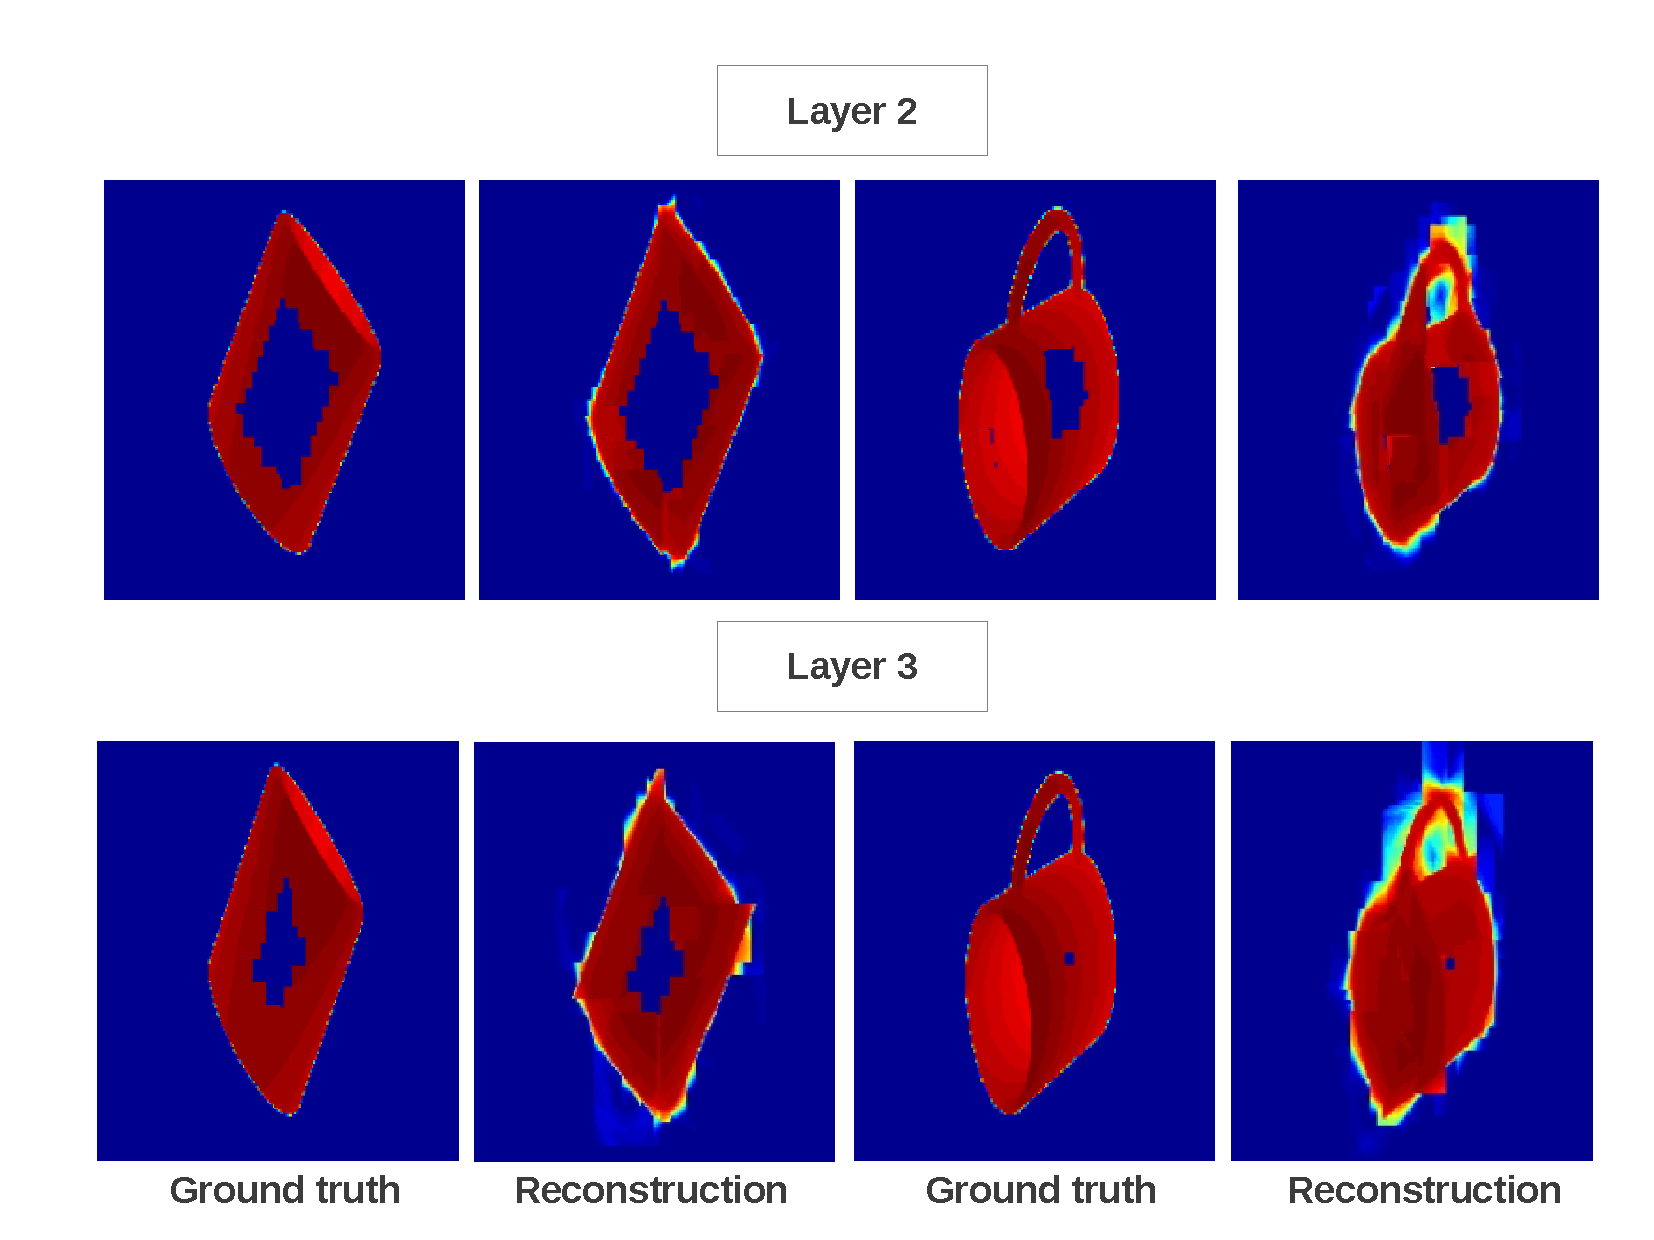
\includegraphics[width=0.7\textwidth]{reconstruction_depth}
\end{center}
\caption{3D view-based reconstruction examples of a mug instance from different viewpoints at Layer 2-3.}
\label{reconstructionDepth}
\end{figure}

Our aim consists in quantifying the predictive power of the learned correspondences between 2D and view-based 3D information channels, at each layer of their compositional representations, aim which is assessed using multiple statistical measures. First, we assess the conditional probabilities of 2D parts given 3D parts and vice-versa and compute the predictive power in the case of choosing the part which maximizes the conditional probability. Some examples of correlations are depicted in Figure \ref{correlations}.

\begin{figure}
\begin{center}
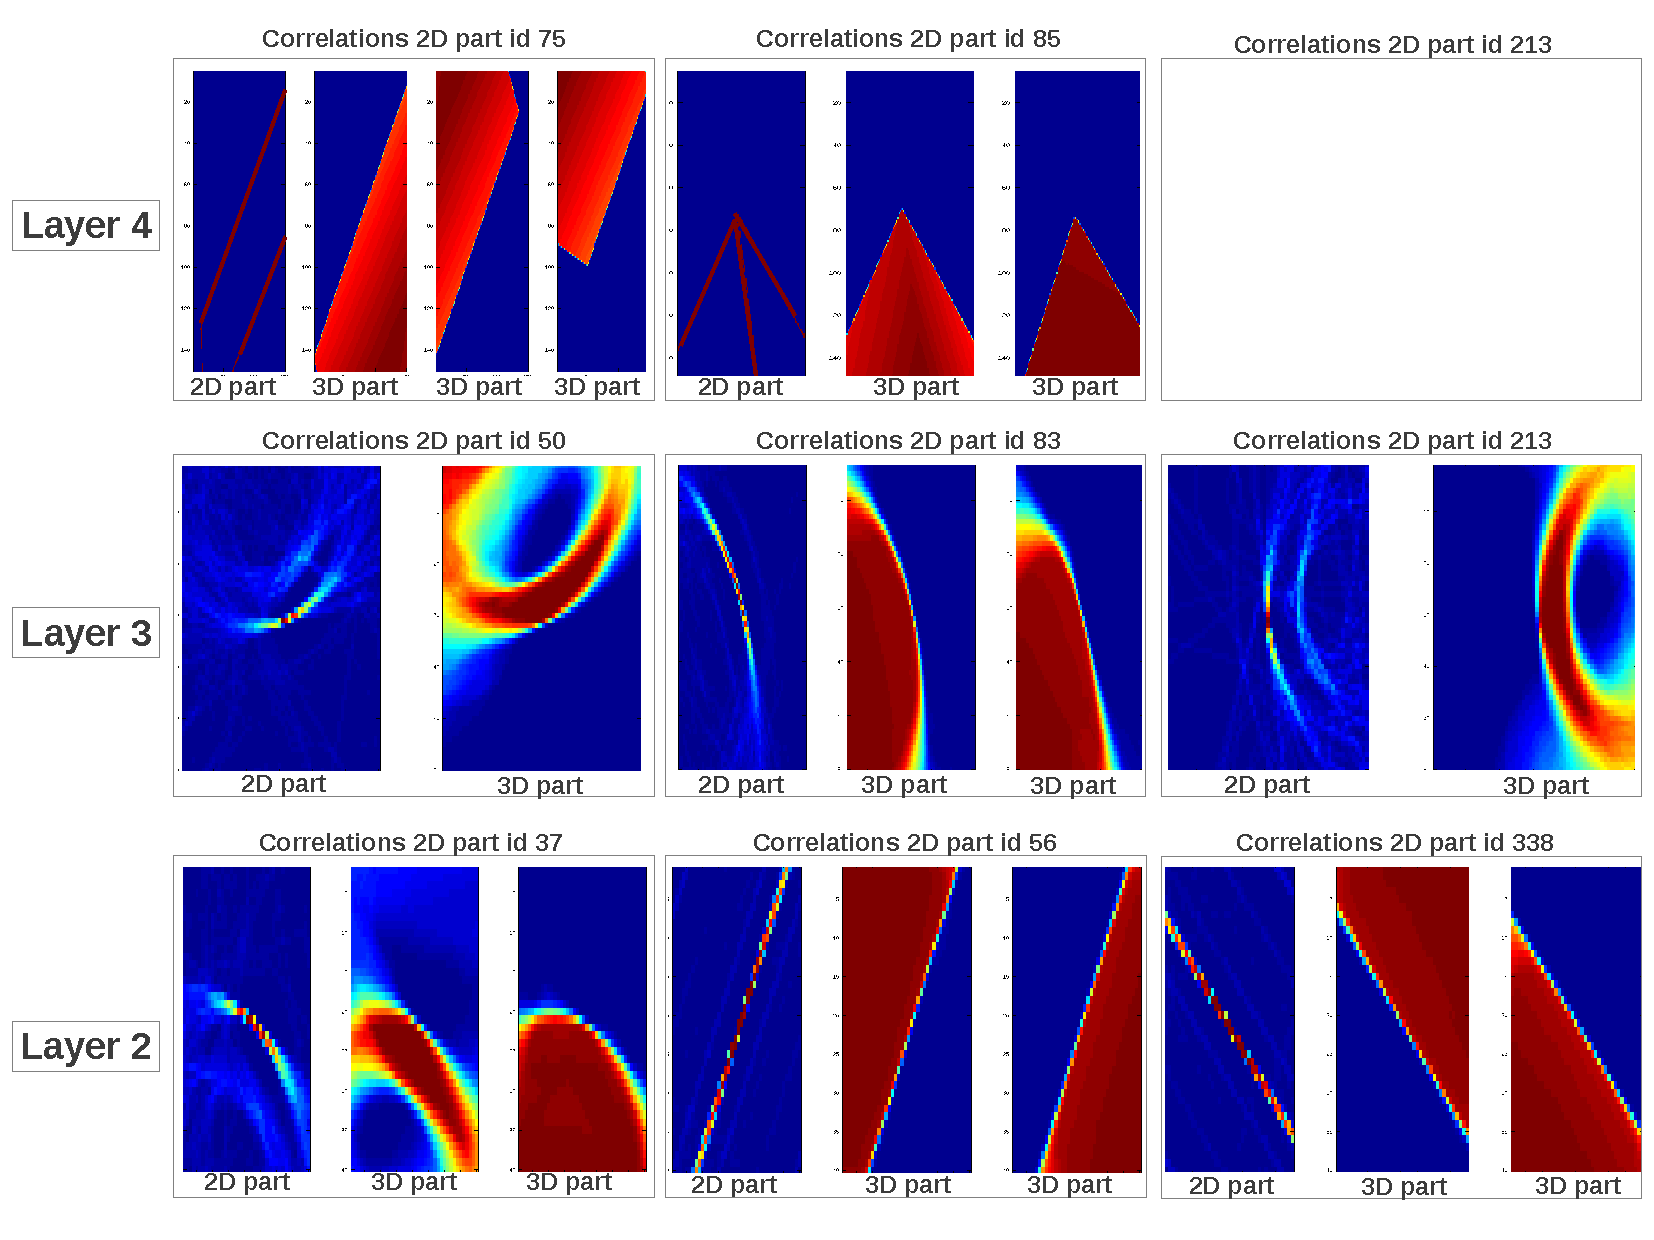
\includegraphics[width=0.8\textwidth]{correlations_1_3}
\end{center}
\caption{Correlation examples between 2D and the best corresponding view-based 3D parts at Layers 2-3.}
\label{correlations}
\end{figure}

As there are many-to-many correspondences, choosing the best part according to the conditional probability is not always the best choice, but only in overall 20\% of the cases, due to ambiguity of edge structures which could correspond to many depth parts. Therefore, one solution for obtaining an efficient inference of view-based 3D parts, given observed 2D parts consists of extracting complementary information from the surrounding region around an edge part using HOG features. Additionally, we trained a k-nearest neighbour classifier for improving the prediction of view-based 3D parts. The obtained results for each layer are presented in Table 2 together with the reconstruction error of view-based 3D parts given 2D parts and statistical measures such as conditional entropy. The cross hierarchy reconstruction error is computed using an adapted version of (8):
 
\begin{equation}
 r_j^l(3D|2D) = \frac{\left\|\Omega_{m'}^l-D_j^l\right\|_2}{\left\|D_j^l\right\|_2}, 
\end{equation}
 where $m'$ is the index which maximizes the conditional probability of a view-based 3D part given the observed 2D part $\Gamma_m^l$ and $D_j^l$ is the ground-truth depth patch corresponding to the observed 2D patch $Z_j^l$ at layer $l$:
 
\begin{equation}
 m'=max_{i=1}^{n_l^{'}}P(\Omega_i^l|\Gamma_m^l)
\end{equation}
and $m$ is the index of best fitting 2D part for the patch $Z_j^l$.
\begin{equation}
 m=min_{i=1}^{n_l}(\left\|\Gamma_i^l-Z_j^l\right\|_2).
\end{equation}

 \begin{table}
 \begin{center}
  \begin{tabular}{ | c | c | c | c | c | c | c |r |}
      \hline
      $Layers$  & $Max Prediction$ & $Err(3D|2D)$ & $K-nn$ & $Err(3D|2D)$ & $H(\Theta^l|\Gamma^l)$ & $H(\Gamma^l|\Theta^l)$  \\ \hline
    $l_1$ &  34.12\% & 1.39 & 50.43\% & 0.64 & 2.51 & 1.93 \\ \hline
    $l_2$ &  27.36\% & 0.99 & 53.6\% & 0.56 & 2.68 & 2.77 \\ \hline
    $l_3$ &  24.27\% & 0.87 &  & 0.44 & 2.92 & 2.63 \\ \hline 
    $l_4$ &  22.44\% &  &  &  & 2.62 & 2.43 \\ \hline
    $l_5$ &   &  &  &  &  &  \\ 
    \hline
  \end{tabular}
\end{center}
\caption{Statistics of inference results of view-based 3D parts given 2D observed parts at Layers 1-5 in the 2D and view-based 3D hierarchies.}
\end{table}

In Figure \ref{inference} we depict several examples of depth images formed of view-based parts inferred from observed 2D parts detected from a corresponding edge image using the probabilistic model introduced in section \ref{sec:inference}. As we use overlapping receptive fields in both hierarchies, we enforce consistency of overlapping predictions using a correlation score for each pixel, weighted by the confidence of the 2D parts that predicted its value and the conditional probability of the view-based 3D part given the observed 2D part. Each pair of images on each layer $l\in\{1,\ldots,5\}$ in Figure \ref{inference} is composed of the ground truth depth image and the predicted one based on 2D parts detected at each specific layer and only contain data around edge parts, while the size of the predicted region is increasing at at each layer.

\begin{figure}
\begin{center}
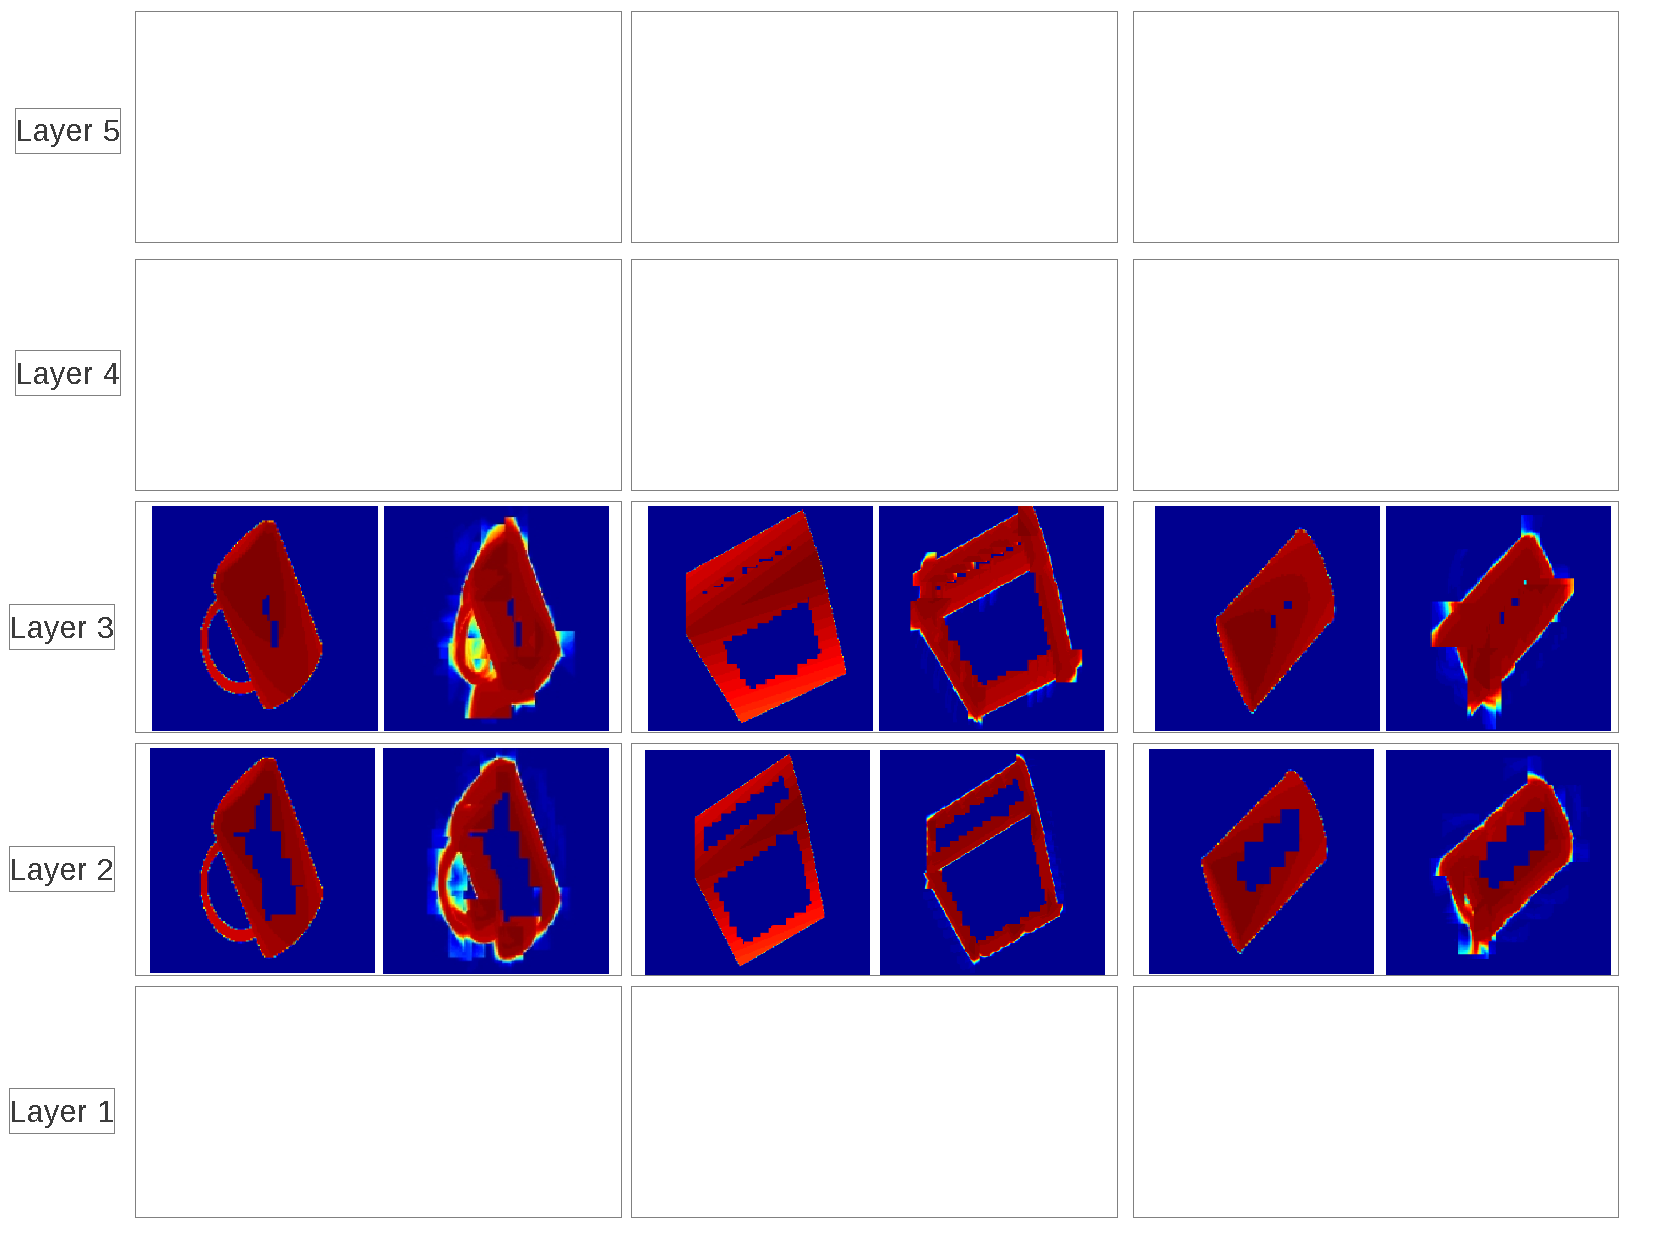
\includegraphics[width=0.8\textwidth]{inference}
\end{center}
\caption{Reconstruction examples of depth images based on inference results of view-based 3D parts given 2D observed parts at Layers 1-5 in the 2D and view-based 3D hierarchies.}
\label{inference}
\end{figure}

\section{Conclusion}
\label{sec:conclusions}
 
In this work we proposed a method for constructing two hierarchical representations, for two information channels, 2D edge images and view-based 3D data. Our model uses as a learning algorithm a sparse autonencoder network, which propagates information from bottom-up, while offering an efficient inference mechanism across hierarchies, based on discretization of each layer responses. 

Next, we evaluated the statistical relationship between representations obtained from 2D and view-based 3D models, analysis which facilitates also the understanding of the geometric properties of the two compositional representations. The evaluation of the learned correspondences between parts in the two hierarchies showed that meaningful correlations can be formed for a set of parts. 

Next, we introduced a probabilistic fusion model for inferring missing observations, by exploiting the correlations between 2D and view-based 3D primitives. The fused model enables an improved and refined representation of the world, by encompassing both 2D and 3D aspects of a scene. Moreover, it facilitates inference of one view from the other, in the case when only one hierarchical representation is available, or under challenging conditions, such as occlusions or noisy sensor data. 

\bibliographystyle{splncs}
\bibliography{egbib}
\end{document}
